184. \begin{figure}[ht!]
\center{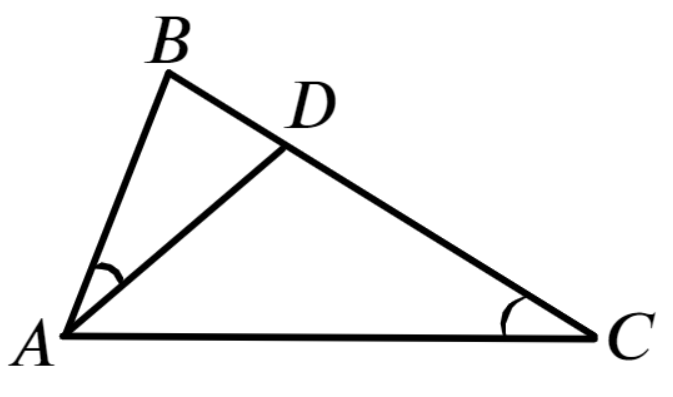
\includegraphics[scale=0.35]{g8-184.png}}
\end{figure}\\
Треугольники $ABC$ и $ABD$ подобны по двум углам $(\angle BAD = \angle ACB,$ угол $B$ --- общий). Поэтому $\cfrac{AD}{AC}=\cfrac{AB}{BC}=\cfrac{BD}{AB},$ то есть
$\cfrac{AD}{8}=\cfrac{4}{6}=\cfrac{BD}{4},$ откуда $AD=\cfrac{16}{3},\ BD=\cfrac{8}{3}.$ Тогда $DC=6-\cfrac{8}{3}=\cfrac{10}{3},\ AC=8,\ AD=\cfrac{16}{3}.$\\
